\documentclass[10pt,a4paper]{article}
\usepackage[utf8]{inputenc}\usepackage[T1]{fontenc}\usepackage[spanish]{babel}
\usepackage{lmodern,amsmath,amssymb,booktabs,graphicx}\usepackage[margin=1.9cm]{geometry}
\usepackage[hidelinks]{hyperref}\setlength{\parindent}{0pt}\setlength{\parskip}{4pt}
\begin{document}\begin{center}{\Large Presupuestos de residuos y protección del costo}\\[4pt]
{\large Sensibilidad exacta y aceptación con certificado}\\[3pt]
14 de octubre de 2026 --- investigación separada de OMS\end{center}
\textbf{Resultado útil.} El diagnóstico ajustado mide cuánto pueden abaratar
el objetivo los presupuestos numéricos. En nive basta reducir los presupuestos
de 40 de 2836 filas, conservando todas las precisiones de cotas continuas,
para proteger el costo al 1\% de un patrón auditado. Diez casos certificados.
No es un presupuesto universal ni una ventaja de solver demostrada.
\section*{Diseño y datos}
Las 72 entregas de los 80 tratamientos previos contienen 41 patrones enteros
distintos: 12 de nive y 29 de los otros cuatro modelos. Los controles fuertes,
solvers y semillas son los anteriores; no se ejecuta otro MILP. Se conservan
ocho ausencias de entrega. L2/Budget de nive repiten patrones por semilla.
El estudio es retrospectivo y control es referencia conocida.

178 LP fijados antes de resolver: $v(0),v(1)$ para los 41 patrones, siete
escalas diádicas intermedias y el umbral de factibilidad para los 12 de nive.
Después se aplicó la regla predefinida: diez umbrales de pérdida al 1\% y diez
validaciones de factor seguro. Una extensión selectiva posterior añadió diez
LP con protocolo separado. Total: 208 llamadas, 2 s por LP y watchdog 4 s.
\section*{Vulnerabilidad potencial del objetivo}
Para enteros $z$ fijados y cotas enteras exactas,
\[
v_z(\lambda)=\min_y\{c_I^\top z+c_C^\top y:\text{filas y cotas continuas
con presupuestos }\lambda\delta,\lambda\beta\}.
\]
Si el patrón es factible exactamente, $D_z(\lambda)=v_z(0)-v_z(\lambda)$.
Mide deterioro potencial; no el error observado en cada salida de un solver.
Se usa $\delta_r=10^{-4}\max(1,|b_r|)$, $\beta_j=10^{-4}$: precisiones
algebraicas experimentales, sin interpretación de tolerancia operativa.
\begin{center}\small\begin{tabular}{@{}lrrr@{}}\toprule
Modelo & Patrones & Inviables & Pérdida potencial (\%)\\\midrule
breastcancer-regularized & 9 & 0 & 0.000038--0.000045\\
control30-3-2-3 & 11 & 0 & 4.816688--7.648345\\
neos-1112787 & 8 & 0 & 0.000917--0.000941\\
neos-3083784-nive & 12 & 2 & 100.000066--100.000142\\
neos-3661949-lesse & 1 & 0 & 0.000000--0.000000\\
\bottomrule\end{tabular}\end{center}
La pérdida se divide por $|v(0)|$ y se muestra como rango de patrones factibles.
En nive, $v(1)\approx-0.0396$: la mínima negatividad procede de ampliar cotas de
no negatividad. No se interpreta como costo físicamente factible o valor nativo.
Control permite deterioros de 4.82--7.65\%, mientras los otros modelos no
muestran esa vulnerabilidad significativa. No se atribuye a los solvers.
\newpage
\section*{Caracterización exacta de nive}
\begin{center}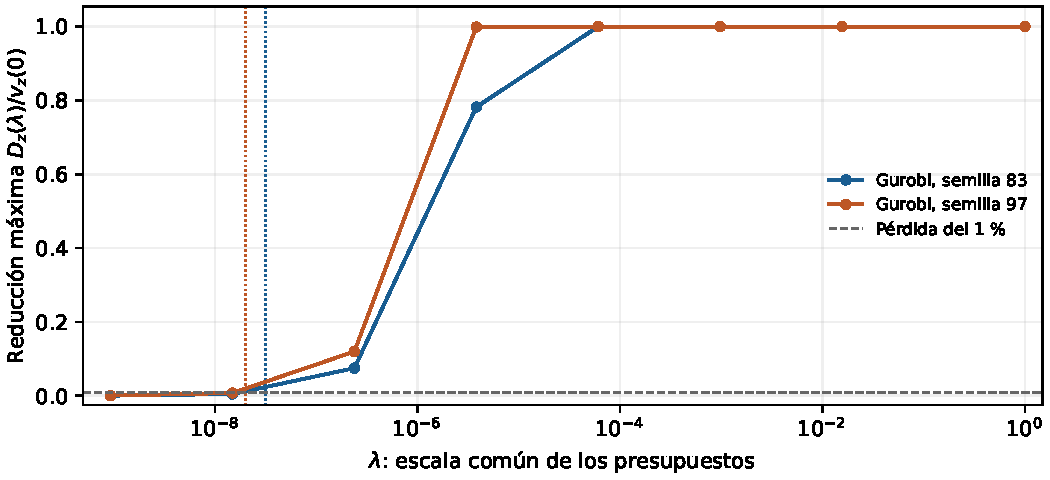
\includegraphics[width=.96\linewidth]{objective-sensitivity.pdf}\end{center}
Puntos: mínimos certificados; líneas: unión visual de muestras, sin garantía
de interpolación. Verticales: primeros presupuestos que permiten una pérdida
del 1\%, con objetivo umbral redondeado hacia arriba a múltiplos de $2^{-40}$.
\begin{center}\small\begin{tabular}{@{}lrrrr@{}}\toprule
Solver & Semilla & $v(0)$ & Umbral $\lambda$ & Factor seguro\\\midrule
Gurobi & 83 & 59631 & 3.18712e-08 & 1/33554432\\
Gurobi & 97 & 37251 & 1.99097e-08 & 1/67108864\\
HiGHS & 83 & inviable & 0.000253768 & --\\
HiGHS & 97 & inviable & 0.000248862 & --\\
\bottomrule\end{tabular}\end{center}
En Gurobi se muestra el umbral de costo. En HiGHS, el de factibilidad:
la mínima ampliación común que permite una continuación del patrón inviable.
No son la misma magnitud ni parámetros de un solver.

Los diez patrones factibles tienen umbrales de costo al 1\% entre
$1.489\,10^{-8}$ y $3.187\,10^{-8}$. El dual fijo y el análisis ajustado dan
los mismos factores diádicos seguros en los diez casos. Un $\Delta$ muy
conservador en $\lambda=1$ puede ser útil cerca de cero; aquí reoptimizar el
dual no permite un factor seguro mayor al nivel de protección elegido.
\section*{Asignación selectiva con protección comprobada}
Con las cotas continuas escritas como filas y dual $\pi\le0$ de $v(0)$,
\[
c(y)\ge v(0)-\sum_i|\pi_i|w_i',\qquad
\sum_i|\pi_i|w_i'\le\varepsilon_{\rm obj}.
\]
Se reduce por el factor seguro solo cada presupuesto $w_i$ con precio no
nulo; los demás se conservan. Una igualdad comparte presupuesto para ambos
lados. Se preservan coeficientes, objetivo, RHS, cotas y dominios originales;
cambia únicamente la región de aceptación numérica.

La primera variante reduce 40/2836 presupuestos de fila (1.41\%) y 396
presupuestos de cota. Diez LP selectivos certifican pérdida menor al 1\%.
Después se conservan todas las cotas: su efecto permitido es aproximadamente 0.0396.
Asignar el margen restante a las filas activas prueba protección con los
certificados existentes, sin otro LP. Basta reducir 40 filas. La regla
conserva 8/12 entregas de patrones factibles y rechaza los cuatro ceros Gurobi.

Los intervalos contractuales son compatibles con la ventana original y la
hipótesis exportada $10^{-6}$ en ambas variantes; no prueba rendimiento.
La garantía requiere el patrón y su certificado. Otros enteros necesitan
otra prueba, incluida su factibilidad exacta.
\newpage
\section*{Filtro de costo frente a reparación exacta}
El filtro mantiene un costo nominal $C$ si existe un testigo exacto del mismo
patrón con costo $U\le C+\varepsilon$, donde
$\varepsilon=\max(10^{-6},|U|/100)$. Garantiza una continuación de costo
no mayor que $C+\varepsilon$. Es unilateral: no acota exceso de costo,
gap u optimalidad global. Si falla, corrige con un testigo comprobado o se abstiene.
\begin{center}\begin{tabular}{@{}lrrr@{}}\toprule
Regla & Conservar entrada & Corregir & Abstenerse\\\midrule
Presupuesto primal solo &72&0&8\\
Reparación exacta, misma cache &28&40&12\\
Filtro de costo, misma cache &64&4&12\\\bottomrule\end{tabular}\end{center}
Las cuatro correcciones del filtro son ceros Gurobi; cuatro abstenciones
adicionales son salidas HiGHS con dos patrones inviables repetidos. Las ocho
ausencias originales siguen contadas. El filtro conserva 36 entradas más
sin activar corrección; no ahorra llamadas para adquirir certificados.
Son acciones del flujo: convertir el testigo racional puede devolver las
mismas coordenadas binary64 del punto original.

Ambos usan 33 adquisiciones por patrón, con 10.355 s
observados. Es imputación retrospectiva sobre candidatos guardados, no un
ensayo end-to-end ni una comparación de velocidad. La reparación ya aporta
la misma existencia de continuación. No se reclama ventaja de trabajo solver.

\section*{Comprobación y alcance matemático}
La ampliación tiene la forma $Ay\le b+\lambda w$, con todas las variables
libres y sus cotas como filas. El checker exige $\pi\le0$, $A^\top\pi=c$,
factibilidad primal exacta e igualdad del costo primal y dual. Un rayo de
inviabilidad debe tener $A^\top\pi=0$, $\pi^\top b>0$. Verifica cada fila
contra los datos originales, sin importar el constructor experimental.

Por dualidad fuerte, optimizar sobre todos los duales factibles da $v(\lambda)$;
mantener un dual de $v(0)$ da una cota suficiente. Restringirse a duales
óptimos en cero no representa toda la sensibilidad global. La función valor
es convexa y no creciente en la región factible; las muestras verifican ambas
propiedades. Los umbrales se obtienen minimizando $\lambda$, con o sin la
fila adicional de costo, y se respaldan con primal/dual exacto.

La sensibilidad, dualidad y reparación racional son herramientas conocidas.
Aquí se mide su utilidad y alcance, sin anunciar un nuevo teorema o algoritmo
MILP globalmente certificado.
\newpage
\section*{Reproducibilidad y resultados adversos}

Se verifican 195 certificados óptimos nativos y 12 rayos.
Un LP de umbral terminó con error numérico, conservado íntegramente. Su
umbral cero se prueba sin repetirlo: primal ya certificado de $v(0)$ y dual
de $\lambda\ge0$. No se cuenta como resolución exitosa.

Las 208 llamadas costaron 87.927 s de ciclos completos; 22.885 s
fueron llamadas al ejecutable y 18.840 s comprobaciones de certificados.
Preparación compartida, replay y documentos se registran aparte. No se
extrapola el promedio a instancias mayores.

Un test detectó antes de cualquier llamada LP una pérdida de coeficientes
en las cotas de $\lambda$ del constructor. Se conservan el diseño anterior y
la corrección pre-solve; muestras y parámetros permanecen iguales. Los
seis tests comprueban signos, estacionariedad, rayos, igualdades, cotas de
$\lambda$ y aceptación del costo, incluidos fallos que exigen abstenerse.

Los racionales corresponden al modelo canónico binary64; todos los literales
originales de nive son exactos en esa representación. Los demás modelos
conservan sus cuentas de redondeo y no se certifica su versión decimal ideal.
El ZIP incluye fuentes, diseños, copias MPS, puntos, logs, primales, duales,
rayos, curvas, presupuestos y tiempos. Binarios y licencias de solver se excluyen.
\section*{Decisión y siguiente barrera científica}
Hay un diagnóstico ajustado y una asignación selectiva comprobable que
protege el costo de patrones conocidos. También hay vulnerabilidad potencial
en control, distinta de un error observado. El filtro evita mantener ceros
sin respaldo y puede conservar entregas suficientemente precisas.

Todavía no hay ventaja algorítmica demostrada frente a reparación exacta
con la misma cache, ni presupuestos preventivos para enteros desconocidos.
La aportación actual no justifica otro paper o una tercera contribución.
Se mantiene OMS v1.3.5 sin cambios, con este estudio independiente.
\section*{Reproducción y fuentes primarias}
\begin{verbatim}
python3 exploration/oms-objective-budget-20261014/independent_check.py
python3 -m pytest -q exploration/oms-objective-budget-20261014/
python3 exploration/oms-objective-budget-20261014/write_report.py
\end{verbatim}
Replay: Python y NumPy, sin solvers; tests: pytest; figura: Matplotlib.
El paquete verifica todos los hashes antes y después, vuelve a generar texto
y figura y recompila este PDF desde una extracción limpia.

\href{https://web.stanford.edu/~boyd/cvxbook/bv_cvxbook.pdf}{Boyd--Vandenberghe,
sección 5.6}: dualidad, perturbación y sensibilidad conocidas.
\href{https://soplex.zib.de/doc/html/EXACT.php}{SoPlex}: LP racional exacto.
\href{https://arxiv.org/abs/2101.09141}{Eifler--Gleixner}: antecedentes de
reparación y certificación racional MILP. Modelos externos:
\href{https://miplib.zib.de/tag_numerics.html}{MIPLIB Numerics}.
\end{document}
